\chapter{ADM}
\section{Introduccción}
El método de desarrollo de arquitectura TOGAF (ADM) forma el core de TOGAF. Es un método confiable y comprobado para desarrollar una arquitectura de TI que satisfaga las necesidades comerciales de una organización. El TOGAF ADM describe el proceso de pasar de la Arquitectura de la Fundación TOGAF a una arquitectura específica de la organización (o conjunto de arquitecturas), aprovechando los elementos de la Arquitectura de la Fundación TOGAF y otros componentes arquitectónicos y bloques de construcción relevantes.

La arquitectura de la Fundación TOGAF no es, por supuesto, el único recurso disponible para el arquitecto al usar el ADM. Existe una amplia gama de modelos arquitectónicos, componentes y bloques de construcción relacionados con diferentes aspectos del dominio de la arquitectura. Este contexto mucho más amplio en el que reside la Arquitectura de la Fundación TOGAF se conoce como el Continuum Empresarial. Es importante tener en cuenta que, al ejecutar el ADM, el arquitecto no solo está desarrollando el resultado final de una arquitectura específica de la organización, sino que también está agregando el propio Continuum empresarial con todos los activos arquitectónicos identificados. 

Aunque el enfoque principal del ADM es el desarrollo de la arquitectura específica de la organización, en un contexto más amplio, el ADM también puede ser visto como el proceso de poblar el  Continuum Empresarial de la organización con bloques de construcción reutilizables.El desarrollo de la arquitectura es un proceso iterativo y continuo, y al ejecutar el ADM repetidamente a lo largo del tiempo, el arquitecto agrega gradualmente más y más del continuo empresarial de la organización.

De hecho, la primera ejecución del ADM a menudo será la más difícil, ya que los activos arquitectónicos disponibles para su reutilización serán relativamente pocos.Sin embargo, las ejecuciones posteriores serán más fáciles a medida que se identifiquen más y más activos de arquitectura, que se usen para agregar al Continuum Empresarial de la organización y, por lo tanto, estén disponibles para su reutilización \cite{TheOpenGroup2001}.

\section{Principios de diseño de arquitectura}
Una arquitectura es un conjunto de elementos (a veces llamados bloques de construcción) representados en un modelo arquitectónico, y una especificación de cómo se conectan estos elementos para cumplir con los requisitos generales de un sistema de información.

Los diversos elementos de una arquitectura especifican los servicios requeridos en un sistema específico de la organización.Existen algunos principios generales que subyacen en el uso del TOGAF ADM para el diseño y el uso exitoso de arquitecturas específicas:

\begin{itemize}
\item Una arquitectura solo necesita especificar los servicios que requiere.
\item Los elementos de una arquitectura pueden especificar uno, más de uno o solo parte de un servicio.
\item Los elementos de una arquitectura deben definirse en términos de estándares relevantes para los servicios que especifican.
\item Los elementos de una arquitectura deben reutilizarse de todas las categorías del Continuo de Arquitectura y deben admitir la reutilización de elementos de solución del Continuo de Solución.
\item Los elementos de la solución (o implementación) deben reutilizarse de todas las categorías del Continuum de soluciones.
\item Se debe seguir una arquitectura, o es inútil: por lo tanto, se recomiendan prácticas formales de gobierno de TI.
\end{itemize}

La especificación de los bloques de construcción utilizando el ADM es un proceso evolutivo e iterativo. Las fases y pasos clave del ADM en los que se desarrollan y especifican los componentes básicos se resumen a continuación y se ilustran en la Figura \ref{bloques}.

\begin{figure}[h!]
	\centering
	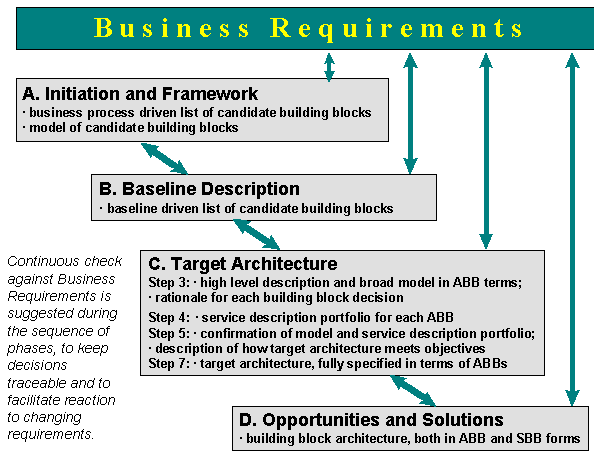
\includegraphics[width=1\linewidth]{ARQUITECTURA/imgs/bloques}
	\caption{Fases clave de ADM en los que se especifican los bloques de construcción}
	\label{bloques}
\end{figure}

\newpage
\section{Adaptación de ADM}

El ADM es un método genérico para el desarrollo de la arquitectura, que ha sido diseñado para hacer frente a la mayoría de los requisitos del sistema y de la organización. Sin embargo, a menudo será necesario ampliarlo para satisfacer necesidades específicas. Una de las tareas antes de aplicar el ADM a una situación específica debe ser revisar la estructura ADM actual y adaptarla si es necesario a las circunstancias de la empresa en cuestión. Esta actividad bien puede producir un ADM específico de la organización. A continuación se listan las razones típicas de adaptación de ADM:

\begin{itemize}
\item Es necesario vincular el ADM con otros procesos, como los de autorización, limitación de riesgos, planificación comercial, presupuestación, planificación del desarrollo, requisitos, gestión de proyectos, desarrollo de sistemas, compras, etc.

\item El ADM se está utilizando como un método de desarrollo para algo que no sea la arquitectura de TI: por ejemplo, arquitectura de aplicaciones, arquitectura de datos, arquitectura empresarial general o como un método general de gestión de programas.Como método genérico, el ADM se adapta bien a este tipo de situaciones.

\item El ADM puede ser utilizado por un contratista principal en una situación de subcontratación, y debe adaptarse para lograr un compromiso adecuado entre las prácticas existentes del contratista y los requisitos de la organización contratante.

\item La organización es una pequeña o mediana empresa, y desea producir un método de reducción más en sintonía con el nivel reducido de recursos y la complejidad del sistema típico de dicho entorno.

\item La organización es muy grande y compleja, y comprende muchas empresas separadas pero interrelacionadas dentro de una metaempresa general, y el método de arquitectura debe adaptarse para reconocer esto. En tales casos, se pueden utilizar diferentes enfoques de planificación e integración.

\item El ADM está dirigido principalmente a arquitectos en organizaciones de usuarios de TI, pero una organización de proveedores cuyos productos están basados en TI podría adaptarlo como un método genérico para el desarrollo de una arquitectura de línea de productos.

\end{itemize}

\newpage
\section{El ciclo de desarrollo de la arquitectura}

Las fases son iterativas, tanto dentro de cada fase como entre ellas mismas .A lo largo de las fases del ciclo, debe haber una validación frecuente de los resultados contra la motivación original para llevar la arquitectura a través de un nuevo ciclo (requisitos comerciales, restricciones financieras y de tiempo, etc.). Esta validación continua, como se muestra en la Figura \ref{cycle}, asegura que la arquitectura satisfaga las necesidades del negocio.

\begin{figure}[h!]
	\centering
	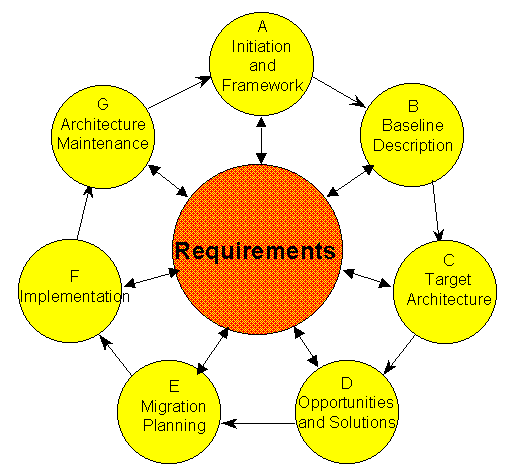
\includegraphics[width=1\linewidth]{ARQUITECTURA/imgs/cycle}
	\caption{Ciclo de desarrollo de arquitectura}
	\label{cycle}
\end{figure}

\newpage
Las fases del ciclo que se muestran en la \ref{cycle} se dividen en pasos, como se muestra en la expansión de la fase de Arquitectura de destino en la \ref{expan}.

\begin{figure}[h!]
	\centering
	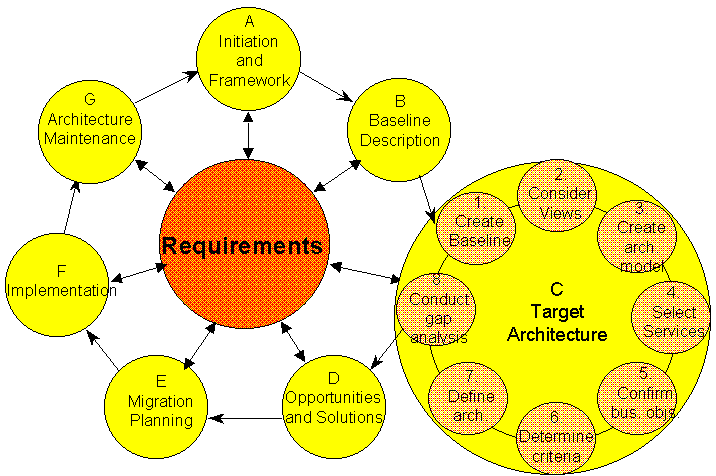
\includegraphics[width=1\linewidth]{ARQUITECTURA/imgs/expan}
	\caption{Expansión del Ciclo de desarrollo de la arquitectura}
	\label{expan}
\end{figure}
